\documentclass{article}

\usepackage[a4paper, portrait, margin=1in]{geometry}

\usepackage[utf8]{inputenc}

\usepackage{todonotes}

\usepackage{graphicx}
\usepackage{hyperref}
\usepackage{lmodern}
\usepackage{xcolor}
\usepackage{float}
\floatplacement{figure}{H}
\usepackage{ragged2e}
\justifying
\usepackage{listings}
%\usepackage{minted}

\title{Data Science in High Energy Physics: How much Higgs?}
\author{Alex Veltman}


\begin{document}

\maketitle

\section*{Introduction}
This tutorial examines the tools and strategies used to compare and build model used when working with particle physics data.
Actual mass distributions of 4-lepton systems from the ATLAS experiment was used as a base to evaluate various models and refine parameter optimisation of models.
Monte Carlo samples of both signal and background sources are used to construct the models assessed.
The tutorial also includes an delve into determining and interpreting the p-value of the data with respect to a model and an investigation into finding the critical value used when determining the 68\% confidence interval of fit parameters when using minimising $\chi^2$.


\begin{figure}
    \centering
    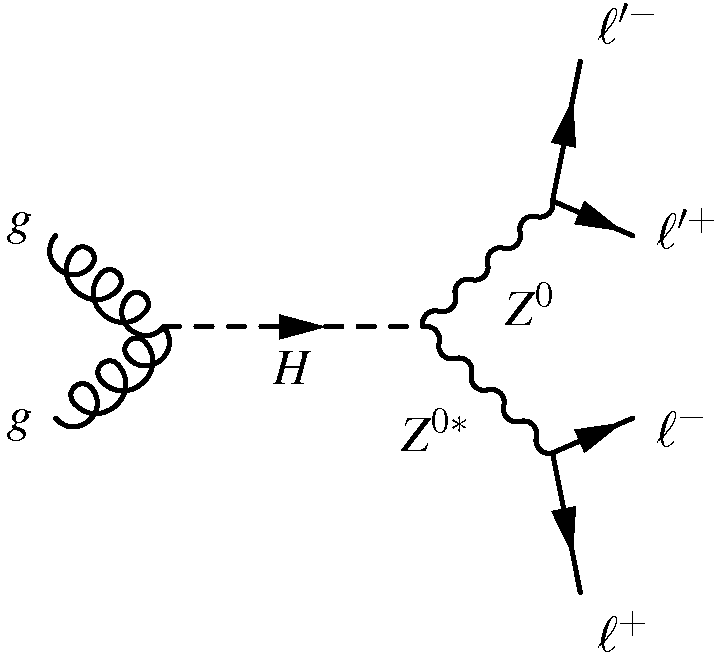
\includegraphics[width=0.3\textwidth]{../hzz.png}
    \caption{Feynmann diagram showing the decay of a Higgs bosons to a two oppositely signed Z boson then to four leptons}
\end{figure}

\section*{Exercise 1}
The model of interest can be seen in Figure~\ref{fig:no_param} where neither the signal nor the background Monte Carlo samples are affected by any scaling factors. \todo{check what stats?}


\begin{figure}
    \centering
    \includegraphics[width=0.7\textwidth]{../no_param.pdf}
    \caption{no param}\label{fig:no_param}
\end{figure}

\section*{Exercise 2}
The one dimensional fit of the $s_s$ parameter produced a best fit value of $s_s= 2.01 \pm 0.76$ minimised the $\chi^2$ value of the data with respect to the model.
The associated uncertainty represents a confidence interval of 68\% about the best fit value.


\begin{figure}
    \centering
    \includegraphics[width=0.5\textwidth]{../s_s_param.pdf}
    \caption{s-s param}
    \label{fig:s_s_param}
\end{figure}

\section*{Exercise 3}
The one dimensional fit of the $s_b$ parameter produced a best fit value of $s_b= 1.302 \pm 0.08$ minimised the $\chi^2$ value of the data with respect to the model.

\section*{Exercise 4}

\section*{Exercise 5}
The $p$-value of the ATLAS data with respect to some $\chi^2$ distribution of a model is calculated with
\begin{equation}
    p(x) = 1 - CDF_{\chi^2(k)}(x)
\end{equation}
where $k$ is the number of degrees of freedom in the model and $x$ is the $\chi^2$ statistic of the data with respect to the model.

The p-value for the fitted model is $0.406$. This indicates that it is very much a possible to obtain data which looks like the ATLAS data from a model with the fitted parameters. The p-value for the model before fitting is $0.015$. The value for the pre-fit model is far smaller than the fitted model which implies that it would be more likely to generate data from the fitted model than it would be to generate the data from the pre-fit model.

If we want to be conservative about our predictions, this simply means that we cannot reject the fitted model.

\begin{lstlisting}[language=Python, numbers=left]
def get_p_value(x, ndf):
    return 1 - stats.chi2.cdf(x, ndf)

chi2_model, ndf = calcChiSq(H_data, means)
chi2_no_model, ndf = calcChiSq(H_data, H_bkg + H_125)

print(get_p_value(chi2_model, ndf-2))
print(get_p_value(chi2_no_model, ndf))
\end{lstlisting}

\section*{Exercise 6}







\end{document}
